\chapter{Geophysics Interferometer (GIF)} \label{chap3}
As shown in Figure \ref{img:img402},  GIF is a 1500 m laser strainmeter installed along the KAGRA X-arm. The laser strainmeter is an asymmetric Michel-son interferometer with 0.5 m and 1500 m arms, which measure the baseline length change of 1500 m relative to the short arm length. The arms are housed in a vacuum chamber, and reflectors are fixed directly to the ground. Therefore, this laser strainmeter can directly measure the baseline length expansion and contraction. Furthermore, we use corner cubes for the reflector to simplify alignment adjustment at the kilometer scale and use no active controls on the optics. This feature makes the stable operation. The GIF has been operating for about three years since it was installed in 2016.

GIF has better low-frequency sensitivity than a seismometer.  Since the seismometer measures the apparent force on its proof mass, it is impossible in principle to distinguish between a tilt component of the ground and the horizontal component of the ground. Moreover, the seismometer also sensitive to the temperature changes in the low-frequency. On the other hand, laser strainmeter does not have such mechanical limitations of seismometers, and the strainmeter can directly measure the expansion and contraction of the baseline length. This chapter compares the sensitivity of GIF and seismometer. The results showed that the GIF had a lower noise level than the seismograph below 0.1 Hz.

In this chapter, instruments of GIF are described. The working principles of the interferometer are described in section \cref{sec:sec42}. Optics of GIF is described in section \cref{sec:sec43}. The realtime signal acquisition system to send the strain signal to KAGRA is described in \cref{sec:sec44}.

\begin{figure}[h]
  \centering
  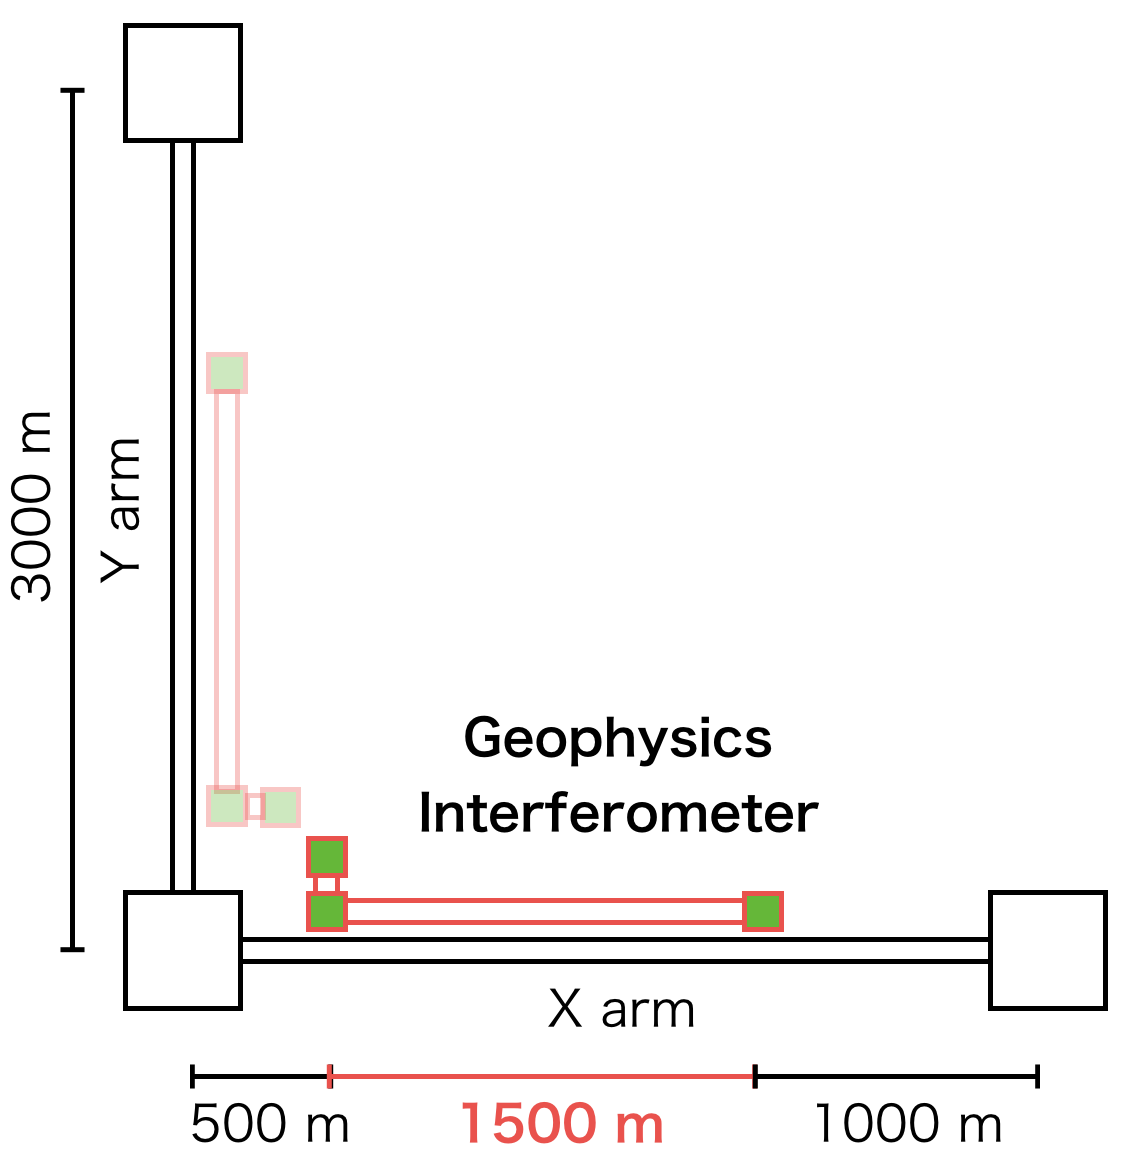
\includegraphics[width=8cm]{./img_chap4/img402.png}
  \caption{Location of geophysics interferometer (GIF). Whereas KAGRA is a symmetric L-shape $3000\,\mathrm{m}$ Michelson interferometer, GIF is an asymmetric $1500\,\mathrm{m}$ Michelson interferometer. GIF is only installed along the X-arm tunnel.} \label{img:img402}
\end{figure}

\section{Working Principle} \label{sec:sec42}
This section describes the measurement principle of GIF and the main noise limiting the strain measurement. GIF is an asymmetric Michelson interferometer with 0.5 m and 1500 m arms. GIF is the equipment that measures the baseline length elongation and contraction of 1500 m based on the short arm length. Therefore, we use the super invar plate whose thermal expansion coefficient is extremely low as the reference arm, and both arms are housed in vacuum tanks so as not to be changed by air fluctuation. The asymmetric arms cause noise coupling from the laser frequency noise. Thus, we have to decrease the noise for precise strain measurement.

This section also describes the difference in the seismic strain response between 1500 m and 3000 m baselines. While the GIF directly measured at 1500 m, it does not directly measure the 3000 m baseline of KAGRA. However, for example, when the base length is expanded or contracted in dc, the fluctuation of 3000 m is two times that of 1500 m. This relation is true below 1 Hz with some assumptions. Therefore, we can measure the baseline length fluctuation of KAGRA by GIF signal in this frequency band. 

As described in section \cref{sec:12}, the working principle of the strain measurement of GIF is the same as the GW detectors. However, the sensitivity of GIF is limited by the laser frequency noise due to the asymmetric optical configuration.


\subsection{Asymmetric Michelson Interferometer}
\begin{figure}[h]
  \centering
  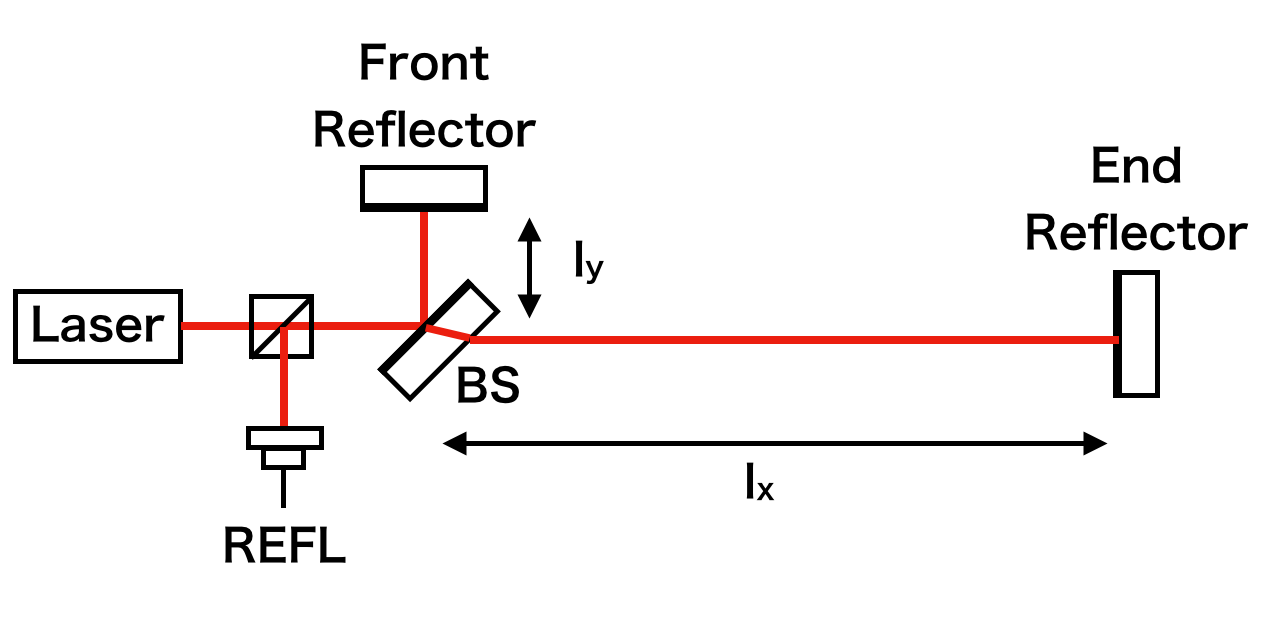
\includegraphics[width=10.0cm]{./img_chap4/img401.png}
  \caption{Schematic drawing of the GIF as an asymmetric Michelson interferometer, which has two different arm lengths, $l_x\gg{l_y}$. In this figure, the mode-matching optics and the optics for signal detection are not drawn.} \label{img:img401}
\end{figure}

An asymmetric Michelson interferometer is an interferometer that is sensitive to both strain changes in baseline length and fluctuations of the laser frequency. Here, consider the Michelson interferometer, as shown in Figure \ref{img:img401}. For simplicity of discussion, it is assumed that the power fluctuation of the laser and the detection noise in the photodetector can be sufficiently ignored. 

The asymmetric interferometer measures changes of baseline length $l_x$ with reference to the short arm $l_y$ and its fringe signal is obtained at the REFL port. The optical phase $\phi_{-}$ is given as
\begin{eqnarray}
  {\phi}_{-} = 4\pi\frac{{l_{-}}}{\lambda}, \label{eq:eq400a}
\end{eqnarray}
where ${l_{-}}=l_{x}-l_{y}$ is the differential of the two arm length and $\lambda$ is the wavelength of the laser. Taking the infinitesimal changes of both side in Eq. (\ref{eq:eq400a}), one can obtain the following equation;
\begin{eqnarray}  
  \Delta \phi_{-} &=& \frac{4\pi}{\lambda}\Delta{l_{-}} - \frac{4\pi}{\lambda^2}\Delta{\lambda}l_{-} \\
  &=& \frac{4\pi{l_{x}}}{\lambda}\left(\frac{\Delta{l_{-}}}{l_{x}} - \frac{\Delta{\lambda}}{\lambda}\frac{l_{-}}{l_{x}}\right) \\
  &=& \frac{4\pi{l_{x}}}{\lambda}\left( \frac{\Delta l_{-}}{l_{x}} + \frac{\Delta f}{f}\frac{l_{-}}{l_{x}}\right), \label{eq:eq400}
\end{eqnarray}
where $\Delta$ denote the infinitesimal change of the variables and $f$ is the laser frequency. 

Consider the asymmetricity of the arms.
Assuming that the X-arm length is sufficiently longer than the Y-arm to be regarded as $\Delta{l_{-}}=l_{x}$, Eq.(\ref{eq:eq400}) can be represented as
\begin{eqnarray}  
  \Delta \phi_{-} = \frac{4\pi{l_{x}}}{\lambda}\left(h  + \frac{\Delta f}{f}\right), \label{eq:eq400_a}
\end{eqnarray}
where $h \equiv \Delta{l_{x}}/l_x$ is the strain of the baseline.

Equation (\ref{eq:eq400}) shows that the optical phase of an asymmetric Michelson interferometer is represented by both the relative fluctuation $\Delta{f}/f$ and the strain of the baseline. Thus, for the interferometer to be sensitive to only the strain, the laser frequency fluctuation must be smaller than the amount of the strain.

\subsection{Noise}
The optical phase must be changed by the baseline length fluctuation. As mentioned above, GIF is an asymmetric Michelson interferometer, so it is sensitive to the laser frequency fluctuations as well as the strain of the baseline. Therefore, a frequency stabilized laser is required. In addition, the optical phase is changed by the fluctuation of the optical path due to a gas in the arms. Thus, the optical path of the interferometer is housed in a vacuum chamber.

\subsubsection{Frequency Noise} \label{sec:123}
As mentioned above, the noise of asymmetric interferometer is limited by the frequency noise because of a lesser amount of common-mode rejection. The GIF, therefore, uses the frequency stabilized laser by using the iodine-absorption line \cite{araya2017design}. The fluctuation $\Delta{f}/f$, which corresponds to the strain, is
\begin{eqnarray}
  h = \frac{\Delta{f}}{f} \sim 7\times10^{-13}.
\end{eqnarray}

\subsubsection{Residual Gas Noise}
GIF interferometer is housed in the vacuum chamber to reduce the residual gas noise. Because residual gas fluctuates the optical path, length measured by interferometer is also fluctuates. The optical path length $L_{\mathrm{opt}}$ is given by $L_{\mathrm{opt}}=nL$, where $L$ is the length of the baseline and $n$ is the refraction index of the medium. Under the pressure of $p$ in vacuum, the index $n$ is approximated as $n = 1 + c_0(p/p_0)$, where $c_0$ denotes the relative refractive index, $p_0$ is pressure in standard air at 1 atm. The apparent strain due to the residual pressure is given as \cite{ciddor1996refractive};
\begin{eqnarray}
  h = (L_{\mathrm{opt}}-L)/L = c_0(p/p_0) \sim 3\times10^{-9} p.
\end{eqnarray}
In order to maintain the strain sensitivity; $3\times10^{-13}$, the vacuum pressure should be below $1\times10^{-4}\,[\mathrm{Pa}]$. However, actual vacuum pressure is $1\times10^{-2}\,[\mathrm{Pa}]$, then apparent strain is $\sim\times10^{-12}$.

\newpage
\subsection{Seismic Strain Response}
In order to use GIF as a baseline length monitor for KAGRA, we should consider the difference in its length. For example, a static baseline length expansion is excited to the baseline lengths of GIF and KAGRA. The strain obtained by dividing each baseline length changes by the baseline length is equal. This relationship is correct when the wavelength of the elastic wave is longer than the baseline length.

\begin{figure}[h]
  \centering
  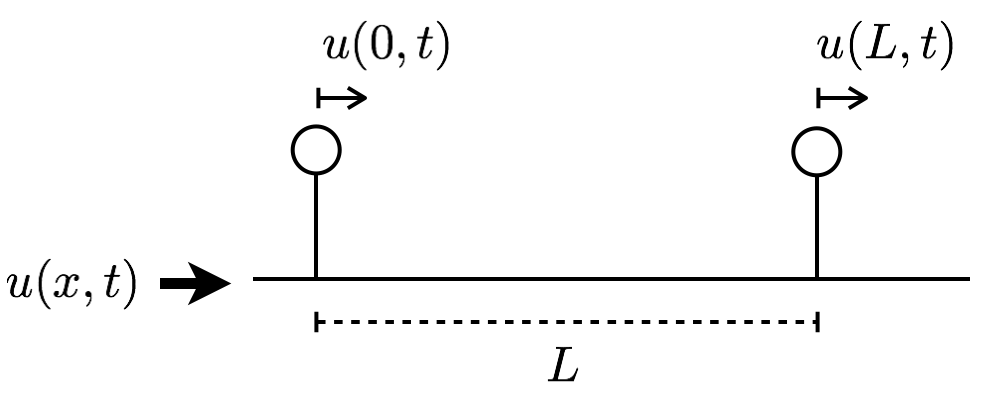
\includegraphics[width=10cm]{./img_chap4/img430.png}
  \caption{Seismic wave propagating two points} \label{img:img430}
\end{figure}

As shown in Figure \ref{img:img430}, consider the response from strain to the optical phase $H_{\mathrm{strain}}$ in the case that the plane seismic waves whose displacement $u(t,x)$ is represented as $u(t,x)=u_0e^{i(\omega{t}-kx)}$ with angular frequency of $\omega$ and the wavenumber of $k$. The seismic wave propagates along with the direction of the baseline (the right direction in this figure).


Relationship between the strain $\epsilon$ and the displacement of the seismic wave $u$ is $\epsilon\equiv{\frac{du}{dx}}$. Relationship between the baseline length change $\Delta{L}$ and the optical phase of the interferometer $\phi_{-}$ is given by $\phi_{-}=\frac{4\pi}{\lambda}$, according to Eq.(\ref{eq:eq400a}). We consider the transfer function from the displacement to the length fluctuation $H_{\mathrm{disp}}$.

\subsubsection{Response from $u$ to $\Delta{L}$, ($H_{\mathrm{disp}}$)}
Before calculating the response to strain, we calculate the response from the displacement of the seismic wave to the baseline length change. First, because the length fluctuation between two mirrors separated with $L$ can be expressed as 
\begin{eqnarray} 
  \Delta{L(t)} &\equiv& u(t,0) - u(t,L) \\
  &=& u(t,0) - u(t-\tau,0), \label{eq:eq403}
\end{eqnarray}
where $\tau=L/v$ is the time delay, the transfer function from the displacement to the length fluctuation is given by Laplace transform as
\begin{eqnarray} \label{eq:eq404}
  H_{\mathrm{disp}}(s) \equiv \frac{\Delta{L(s)}}{u(s)} = \frac{u(s)\left[ 1-\exp(-\tau{s}) \right]}{u(s)} = 1 - \exp(-\tau{s})
\end{eqnarray}

\subsubsection{Response from $\epsilon$ to $\phi_{-}$, ($H_{\mathrm{strain}}$)}
Because the strain amplitude $\epsilon{(x,t)}$ is defined as $\epsilon{(x,t)}\equiv\frac{du}{dx}$, the seismic strain is represented as 
\begin{eqnarray} 
  \epsilon{(x,t)} \equiv \frac{du}{dx} = \frac{du}{dt} \frac{1}{v} = \frac{s}{v}u(s) \label{eq:eq406}
\end{eqnarray}
Therefore, the transfer function from the seismic strain to the displacement is given  as
\begin{eqnarray} \label{eq:eq407b}
  \frac{\Delta{L(s)}}{\epsilon(s)} = H_{\mathrm{disp}} \frac{v}{s}
\end{eqnarray}
Finally, because the transfer function from the length change of the baseline to the optical phase is given as $4\pi/{\lambda_{{}}}$, the transfer function from the seismic strain to the optical phase is represented as 
\begin{eqnarray} \label{eq:eq407}
  H_{\mathrm{strain}}(s) = 4\pi\frac{1}{\lambda_{{}}} \left[1 - \exp(-\tau{s}) \right]\frac{v}{s}.
\end{eqnarray}

Block diagram of the transfer function from the starin to the optical phase $H_{\mathrm{strain}}$ is shown in Figure (\ref{img:img411}). 

\begin{figure}[h]
  \centering
  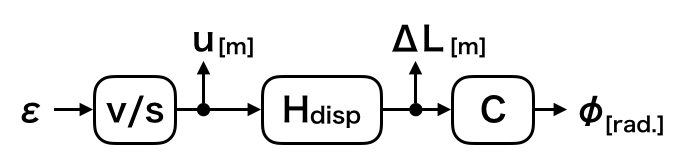
\includegraphics[width=10.0cm]{./img_chap4/img411.png}
  \caption{The response from seismic strain to optical phase.} \label{img:img411}
\end{figure}

\subsubsection{Comparison with the baseline length}
Here, we describe the length dependence of the response given by Eq.(\ref{eq:eq407}). The bode plot of the strain response with two different baseline lengths is shown in Figure  \ref{img:img411_a}. The response has a flat response below the corner frequency defined by 
\begin{eqnarray}
  f_0 = \frac{v}{L},
\end{eqnarray}
where $v$ is the phase velocity and $L$ is the length of the baseline. Thus, if the baseline length is twice, the frequency becomes a half value, which means a decrease of the observation frequency band. For example, in the case of $L=1500\,\mathrm{m}$, and assuming the phase velocity of $5.5 \mathrm{km/sec}$, the corner frequency is $f_0\sim3.7\,\mathrm{Hz}$. In the KAGRA case, the frequency is $f_0\sim1.8\,\mathrm{Hz}$. Therefore, below 1 Hz, the response of both baseline is flat response. In this region, the baseline length fluctuation of KAGRA $\Delta{L_{\mathrm{KAGRA}}}$ is given by
\begin{eqnarray}
  \Delta{L_{\mathrm{KAGRA}}} = 3000\times\epsilon_{\mathrm{GIF}},
\end{eqnarray}
where $\epsilon_{\mathrm{GIF}}$ is the strain measured by GIF in 1500 m baseline.


\begin{figure}[h]
  \begin{center}
    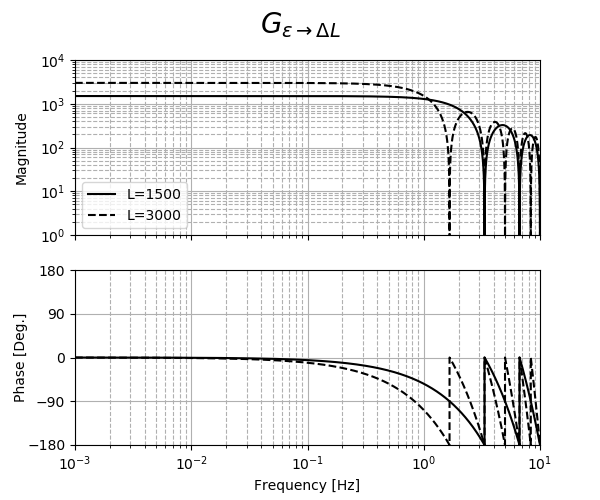
\includegraphics[width=13.0cm]{./img_chap4/img412.png}
    \caption{Compasison of the transfer function from strain of the baseline $\epsilon$ to the length change of that $\Delta{L}$ in the different baseline length given in Eq. (\ref{eq:eq407}) assumed the phase velocity of 5.5 km/s.}\label{img:img411_a}
  \end{center}
\end{figure}

\section{Optics} \label{sec:sec43}
In the previous discussion, the laser light was implicitly assumed the plane wave, which does not change the optical phase and radius of the beam when it propagates, but the actual beam is not. The actual beam requires a design of these beam profiles to interfere with the beam within a finite scale. In this section, we assume a Gaussian beam and describe the design for the GIF interferometer.

\begin{figure}[h]
  \begin{center}   
    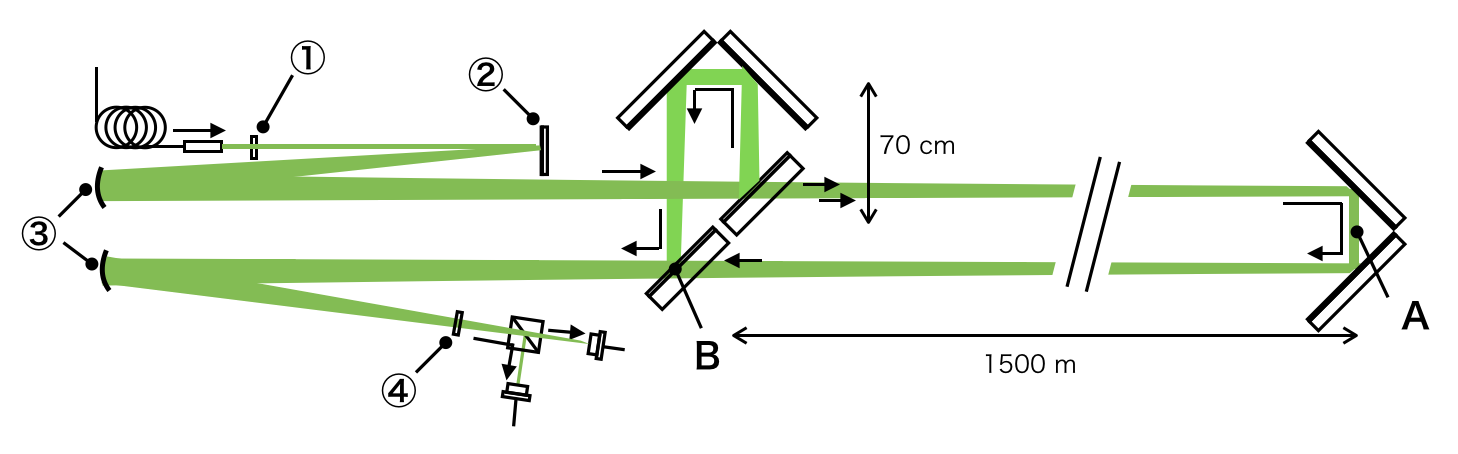
\includegraphics[width=14cm]{./img_chap4/img416.png}
    \caption{Schematic optics layout. (1) A collimator lens for input beam. (2) A flat mirror for steering mirror. (3) Two concave mirrors with a radius of curvature of $9.8\,\mathrm{m}$ for mode matching. (4) A collimator lens for output beam. The waist of the beam is at the end reflector at point A. Two reflected on the reflectors are combined at point B.}\label{img:img416}
  \end{center}
\end{figure}


\subsection{Input Output Optics}
Input-output optics is used for matching the beam profile of the input laser with that of the interferometer in order to interfere, as shown in Figure \ref{img:img416}. The output beam from the laser incidents into a beam splitter (BS) using (1) a collimator, (2) steering mirror, and (3) concave mirrors in order to be the beam waist at the end reflector. The reflected beams from each reflector are re-combine at Point B, and this interfered light is incidents to the photodetector through another concave mirror and collimator. The mode matching is described in reference \cite{miyo2017baseline}.

\subsection{Core Optics}
The core optics of the Michelson interferometer are composed of two reflectors and a beam splitter (BS). The core optics are housed in a vacuum tank not to be affected by environmental changes.  These optics are fixed on the super-invar plate so that the length does not change in temperature. Furthermore, the reflector uses corner cubes. Thus we do not require alignment on the km scale. The vacuum tank containing these optical elements is placed on granite directly fixed to the ground. 

\begin{figure}[h]
  \begin{minipage}[b]{0.5\hsize}
    \begin{center}   
      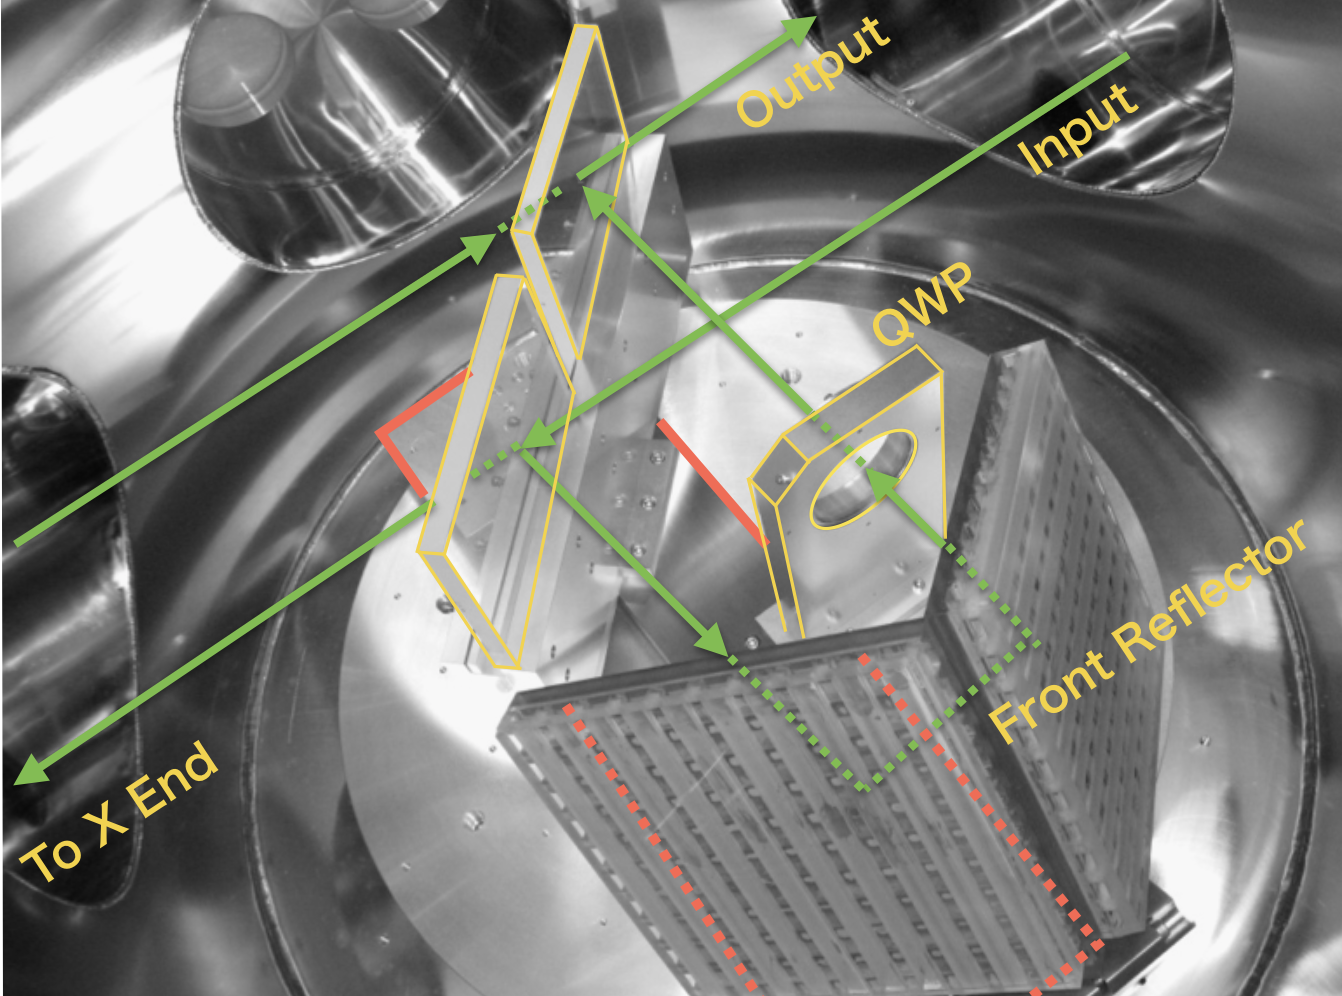
\includegraphics[width=7cm]{./img_chap4/img418.png} % ファイル重い
      %
\includegraphics[width=7cm]{./img.png}
      \subcaption{Core optics in the front vacuum chamber.}\label{img:img418}
    \end{center}
  \end{minipage}\hspace{0.1cm}
  \begin{minipage}[b]{0.5\hsize}
    \begin{center}   
      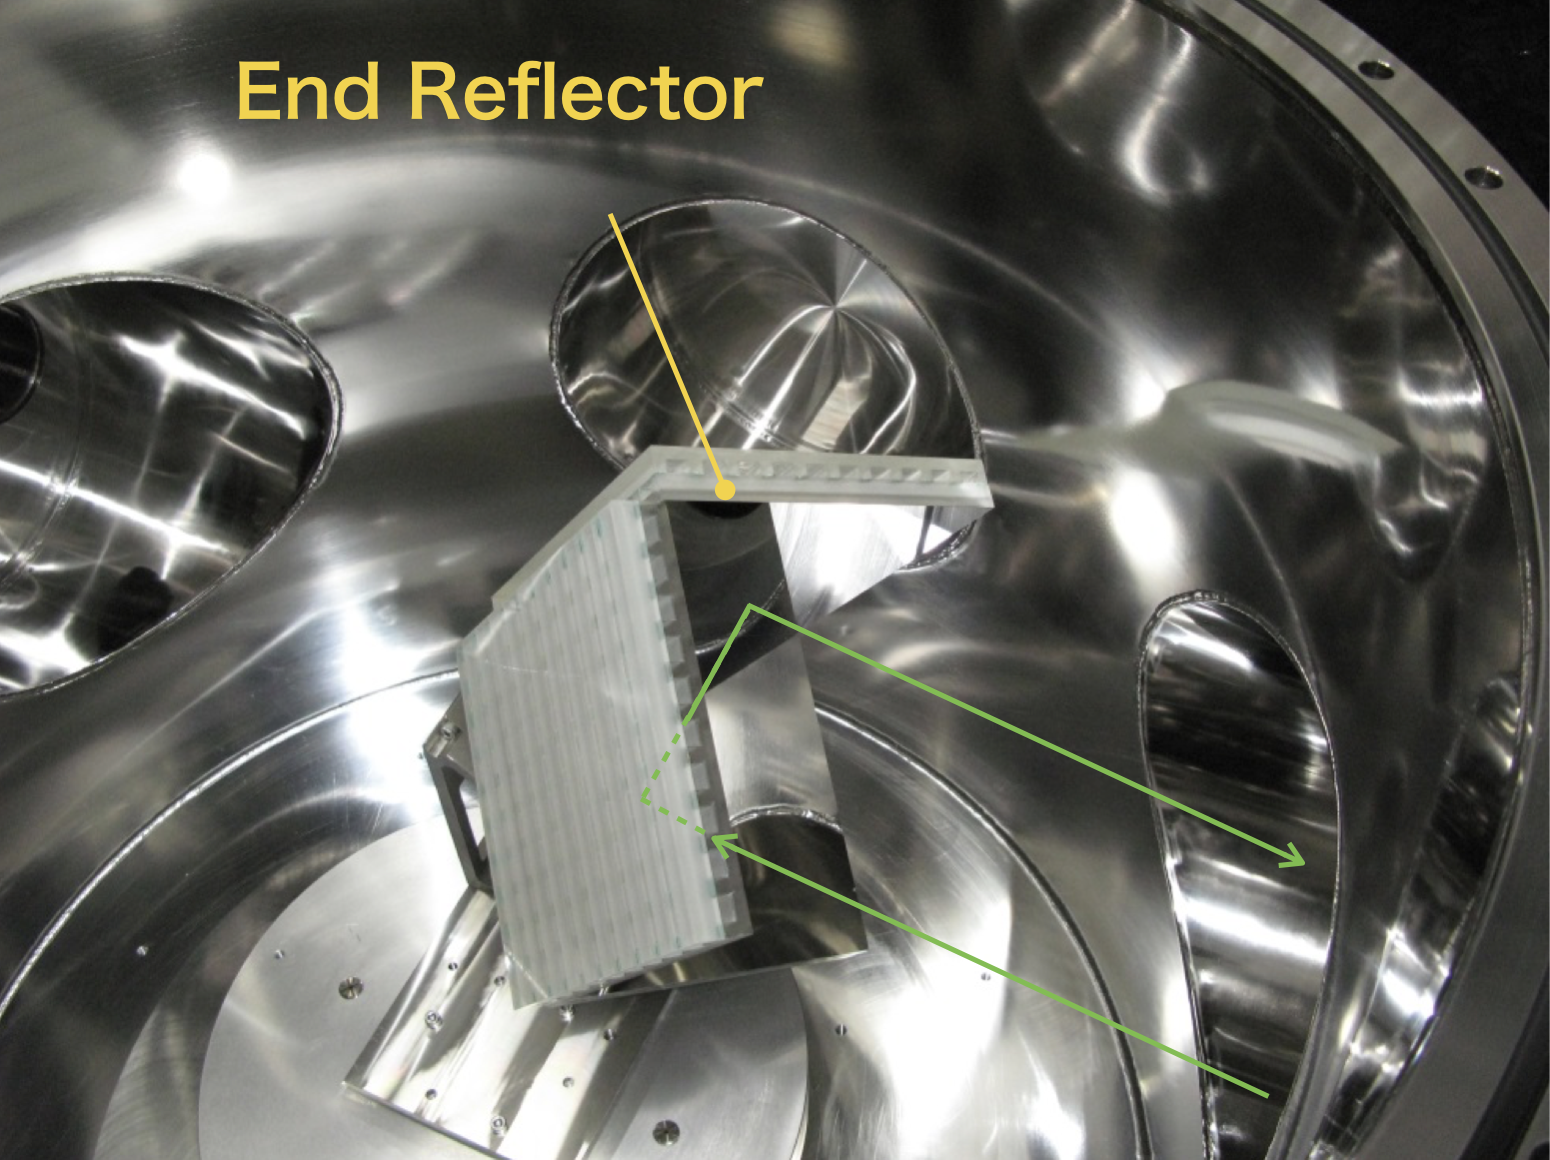
\includegraphics[width=7cm]{./img_chap4/img419.png} %ファイル重い
      %
\includegraphics[width=7cm]{./img.png}      
      \subcaption{Core optics in the end vacuum chamber.}\label{img:img419}
    \end{center}
  \end{minipage}
  \caption{The picture of the core optics.}  
\end{figure}


In order to minimize the size of the reflectors, the beam of the GIF interferometer is designed so that the beam waist is in the end reflector, as shown in Figure \ref{img:img416}. In this case, if the beam waist $w_0$ is focused at the end reflector, the beam radius at the front reflector $w(L)$, which locates 1500 meters from the end reflector, spreads. Therefore, we need to design the beam so that
\begin{eqnarray}
  \argmin_{w_0} \left[w_0\times\frac{w(L)}{w_0}\right]. \label{eq:eq415_e}
\end{eqnarray}
Substituting Eq.(\ref{eq:eq415_b}) into Eq.(\ref{eq:eq415_e}), one can obtain the beam waist radius
\begin{eqnarray}
  w_0 = \sqrt{\frac{{L\lambda}}{\pi}} \label{eq:eq415b}
\end{eqnarray}
We note that the Rayleigh range is $z_0 = L$ in the case of that.

According to Eq.(\ref{eq:eq415b}), the beam waist radius of the GIF is
\begin{eqnarray}
  w_0=\sqrt{{1500\,\mathrm{[m]}}\times 532\,\,\mathrm{[nm]}/\pi} = 16\,\mathrm{mm}.
\end{eqnarray}
Furthermore, the beam radius at the front reflector is $w(1500)=\sqrt{2}{w_0}$. Finally, we determine the size od the reflectors as the three times of the $w(1500)$, then the minimum size of the reflector is $2\times3\times\sqrt{2}w_0\sim270\,\mathrm{mm}$.


\subsection{Frequency Stabilized Laser} \label{sec:sec135}
As mentioned in \cref{sec:123}, because the frequency noise of the laser limits the sensitivity of the strain measurement, the GIF interferometer uses the frequency stabilized laser utilizing the iodine absorption line \cite{araya2002iodine}. The control diagram of the frequency stabilization system is shown in Figure \ref{img:img417}. This control is a feedback system in order to reduce the error signal of the laser frequency and the frequency of the iodine absorption line. The error signal is obtained by the saturated absorption spectroscopy method from the absorption signal that is a doppler free signal by using the pump and probe light \cite{snyder1980high}.
\begin{figure}[h]
  \begin{center}   
    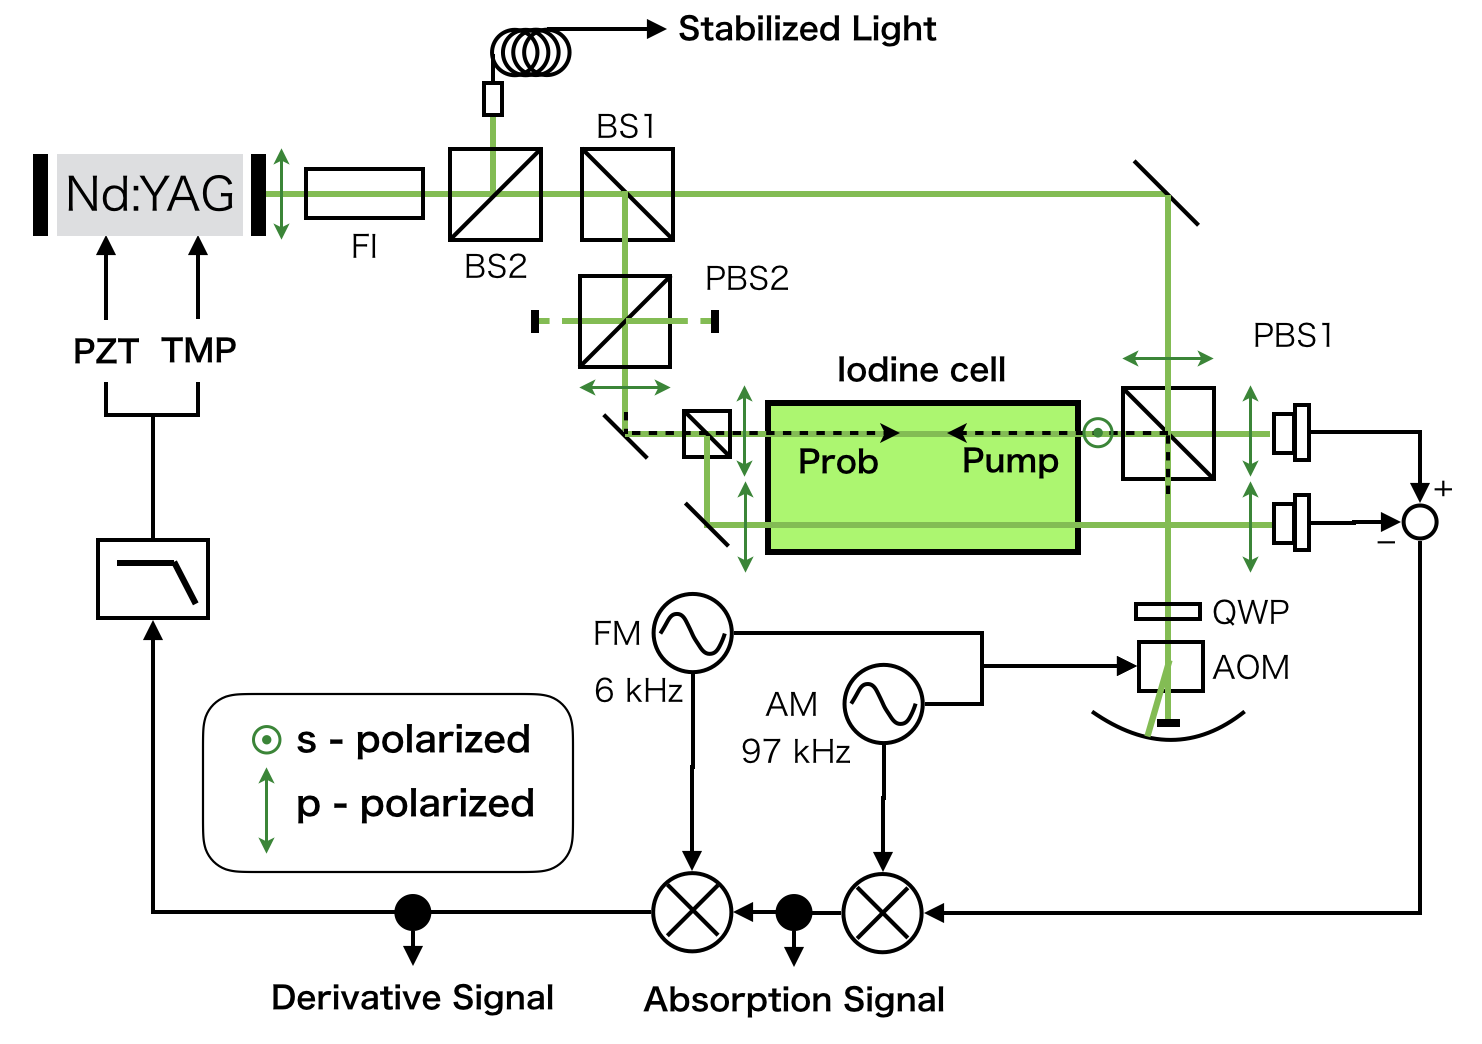
\includegraphics[width=12cm]{./img_chap4/img417.png}
    \caption{Schematic diagram of the frequency-stabilization system of the GIF main laser.}\label{img:img417}
  \end{center}
\end{figure}


\subsection{Quadrature Phase Fringe Detection} \label{sec:141}
\begin{figure}[h]
  \begin{center}
    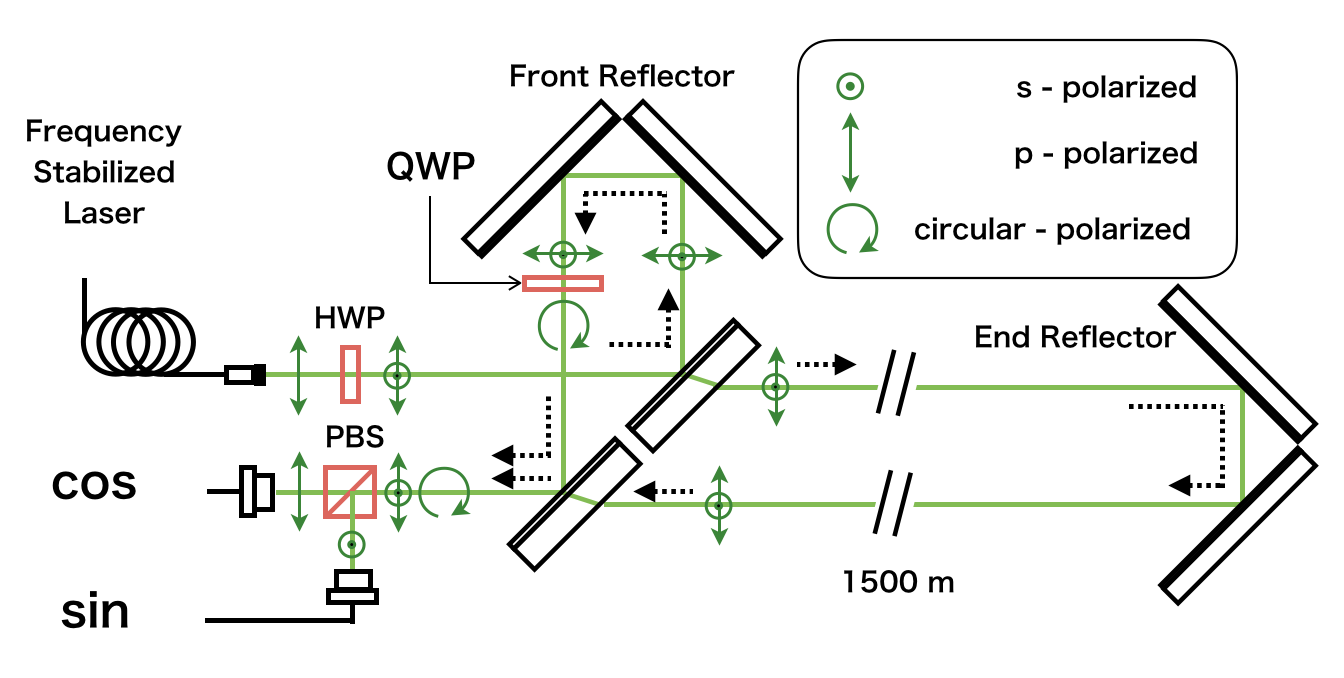
\includegraphics[width=13.0cm]{./img_chap4/img413.png}
    \caption{Quadrature interferometer used in the GIF strainmeter.}\label{img:img413}
  \end{center}
\end{figure}
We use the quadrature-phase fringe detection to measure the length change of the baseline with a wide dynamic range \cite{bobroff1993recent}. The optical layout for the detection is shown in Figure  \ref{img:img413}. A half-wave plate (HWP) produces a p-polarization and s-polarization. A quarter-wave plate (QWP) delay the optical phase of the s-polarized light with 90 degrees against the other. As a result, one can obtain the quadrature-phase fringes.

The quadrature-phase fringes are detected by two photodetectors, these can be represented as 
\begin{eqnarray}
  x(t) &=& x_0 + b \cos(\phi(t)), \label{eq:eq450b} \\
  y(t) &=& y_0 + a \sin(\phi(t)+\delta), \label{eq:eq450a}  
\end{eqnarray}
where $x$ and $y$ are the two voltage outputs from the detectors, $a$ and $b$ are the amplitudes of these fringe signals, $x_0$ and $y_0$ are the offsets, $\phi$ is optical phase, and $\delta$ is the phase offsets from imperfections \cite{zumberge2004resolving}. Here, the optical phase $\phi$ is given by
\begin{eqnarray}
  \phi = \arctan {\frac{\bar{Y}}{\bar{x}}} \label{eq:eq440c}
\end{eqnarray}
where 
\begin{eqnarray}\label{eq:eq440a} 
  \bar{Y} = \left(\frac{\bar{y}-\bar{x}\sin{\delta}}{\cos{\delta}}\right), \\
  \bar{x} = \frac{x-x_0}{b}\,\,\mathrm{and}\,\,\bar{y} = \frac{y-y_0}{a}. \label{eq:eq440b}
\end{eqnarray}
According to Eq.(\ref{eq:eq450b}) and Eq.(\ref{eq:eq450a}), if these parameters are given in at time $t$, the optical phase $\phi(t)$ is obtained.


\section{Realtime Data Aquisition System} \label{sec:sec44}
Essentially, the GIF is an independent instrument from the KAGRA not to interfere with each other. Therefore, the data acquisition system of each was developed independently. However, in order to use the GIF strainmeter for the baseline compensation system, we need to implement the GIF system into the KAGRA system. 

In this section, the realtime data acquisition system is described. In the quadrature-phase detection method, we need the ellipse fitting to obtain the optical phase. In section \cref{sec:142}, the realtime data acquisition system is described. This system process the fitting below $1\,\mathrm{msec}$.

\subsection{Realtime Data Processing} \label{sec:142}
All the PD signals of the GIF are taken by the analog-digital-converter (ADC) and processed in the KAGRA digital system, which is the same as LIGO \cite{bork2001overview}. The ADC converts the analog signal to the digital signal with 16 bit and $2^{16}\,\mathrm{Hz}$ sampling frequency. All the digital signals are simultaneously sampled in the digital system. 

The realtime calculation model in the KAGRA system is shown in Figure  \ref{img:img420}. To reduce the calculation cost, the digital signal in this model is downsampled to $2^{14}\,\mathrm{Hz}$. This realtime model has three main functions; the ellipse fitting function, the strain calculator function, and the unwrap function. These functions are described below.
\begin{figure}[h]
  \centering
  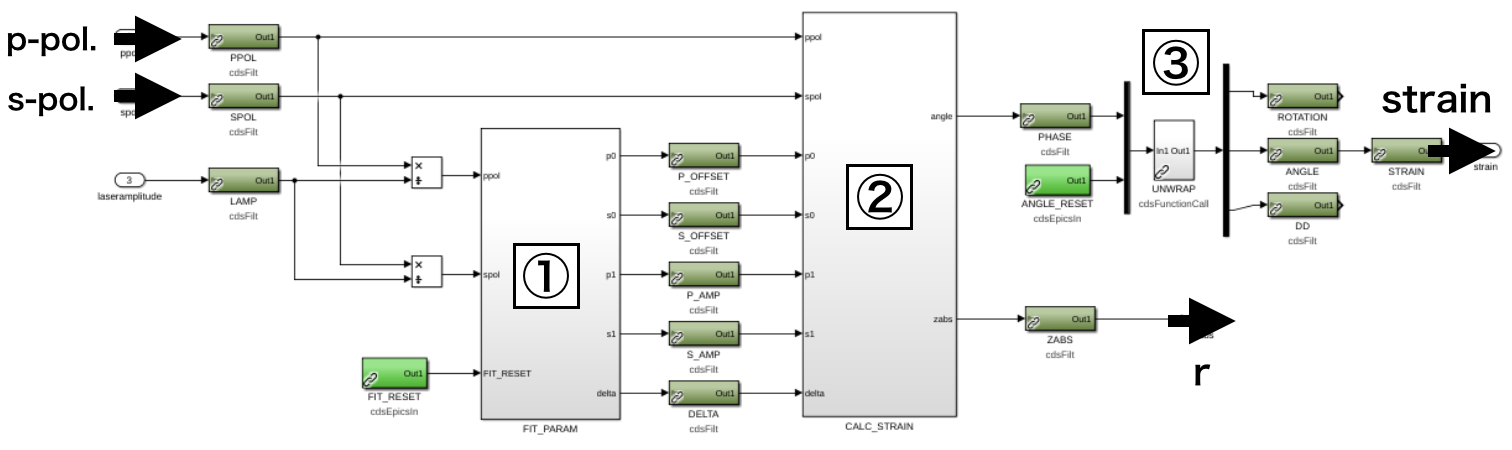
\includegraphics[width=15.0cm]{./img_chap4/img420.png}
  \caption{Realtime calculation model of the phase calculator of GIF. (1) the elipse fitting function (2) the strain calclator function (3) the unwrap function.}\label{img:img420}
\end{figure}

\begin{figure}[h]
  \centering
  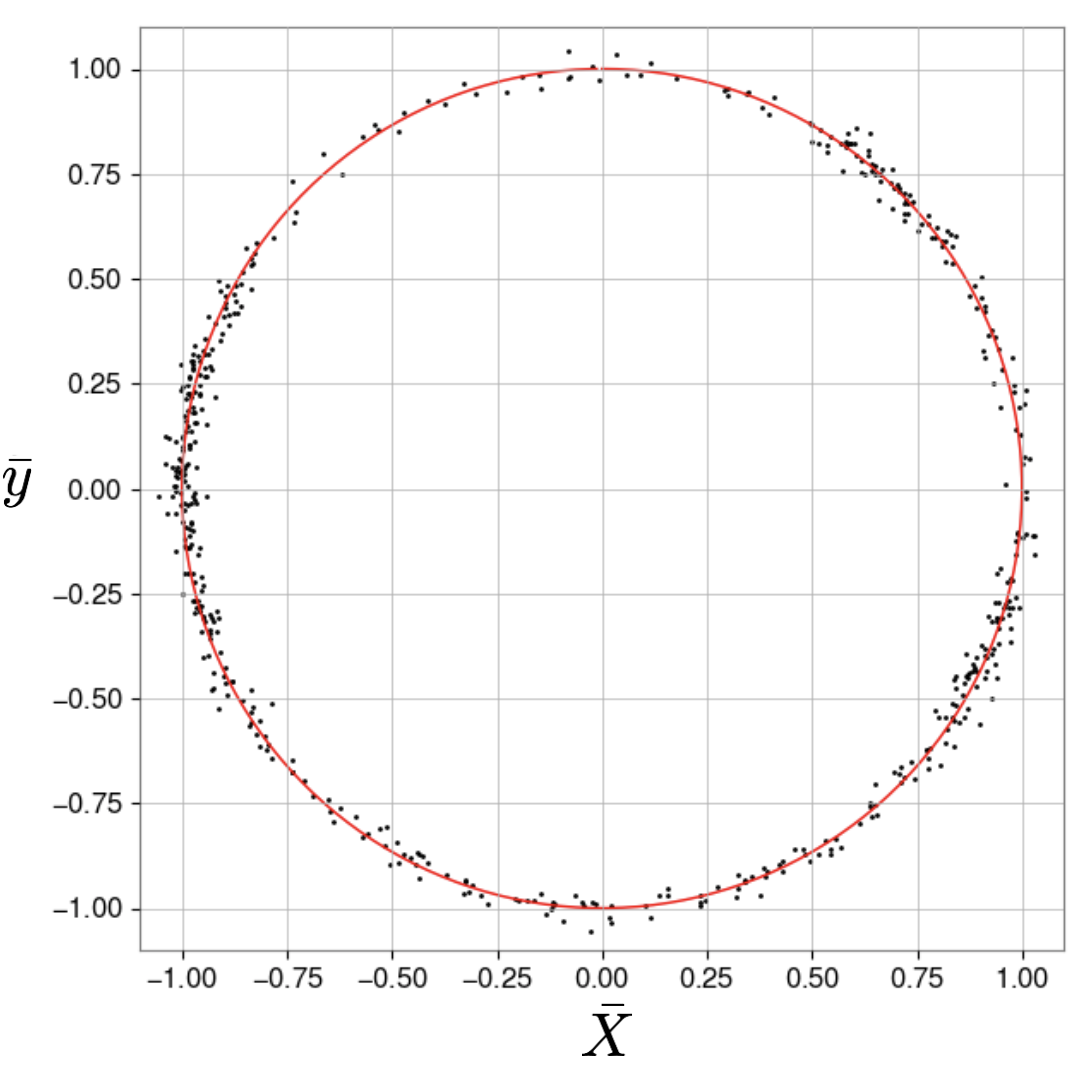
\includegraphics[width=10cm]{./img_chap4/img440.png}
  \caption{Fitting the elipse curve to the Lissajous figure. $\bar{Y}$ and $\bar{x}$ are defined in Eq.(\ref{eq:eq440a},\ref{eq:eq440b}), respectively. } \label{img:img440}
\end{figure}

\subsubsection{Elipse fitting function}
This function is for obtaining the five ellipse parameters in Eq.(\ref{eq:eq450a}) and Eq.(\ref{eq:eq450b}) by fitting the ellipse curve to the Lissajous figure drawn by two PD signals. The function calculates these parameters using the least-square method with 512 data points of each two PD signals, as shown in Figure \ref{img:img440}.

\subsubsection{Strain calculator function}
This function calculates the optical phase using the ellipse parameters based on Eq.(\ref{eq:eq440c}). For example, Figure  \ref{img:img440} shows the fitted curve (red line) and the data points (black dots). As described above, the optical phase $\phi$ is an angle of the data point. This optical phase depends on the power ratio $\bar{y}/\bar{x}$ and the phase offset $\delta$ because the phase is given by
\begin{eqnarray}
  \phi = \frac{\bar{y}}{x}\frac{1}{\cos{\delta}} - \tan{\delta}.
\end{eqnarray}
%({\color{red}{数式が違う。tanがない。数式を丁寧に説明。}})
This means that the changes in the power ratio and the phase offset are the noise of the optical phase measurement. In particular, the power ratio is sensitive at the PBS, which divides the interfered two polarized lights. For this reason,  we covered this location with a small house to protect winds disturbed by passengers. On the other hand, the phase offset has small fluctuation because the QWP is installed in the vacuum chamber.

Although the calculation of the optical phase by measuring the angle is not affected by the input power changes, the signal to noise ratio will worse in less input power. We also monitor the quality of the calculation using a parameter;
\begin{eqnarray}
  r = \sqrt{\bar{x}^2+{\bar{Y}^2}}.
\end{eqnarray}

\subsubsection{Unwrap function}
This function unwraps the optical phase calculated by the phase calculator function and returns the continuous phase proportional to strain because the atan2 function is used in the phase calculator return between $-\pi$ to $\pi$. 

\subsection{Comparison with seismometers}
We measure the 3 km baseline length change by using the seismometers and GIF, and compare their sensitivity. The two seismometers are installed on the corner area and X-end area, which is separated 3 km. The displacement is calculated by the differential signal of the X direction of these seismometers. On the other hand, because the GIF strainmeter directly measures the displacement of the 1.5 km baseline. Thus, the displacement of the 3 km is calculated by this strainmeter signal multiplied factor 2.

Figure \ref{img:img319_a} shows the ASDs of the displacement of the baseline measured by two seismometers and GIF strainmeter. Above 0.1 Hz, seismometer could measure the displacement, but below this frequency, this is limited by self-noise, which increases in low-frequency. On the other hand, a strainmeter could measure the displacement below 1 Hz. For this reason, we use GIF strainmeter to measure the deformation of the baseline in the low-frequency region, which are the main disturbances degrading the duty cycle of GW detectors.

\begin{figure}[h]
    \begin{center}   
      \includegraphics[width=13.0cm]{./img_chap3/img319_a.eps}
      \caption{Baseline length fluctuation measured by two seismometers (black) and GIF strainmeter (green).}\label{img:img319_a}
    \end{center}
\end{figure}



%% \section{Summary of the Chapter}
%% ({\color{red}{簡潔に述べる。箇条書きはだめ。}})
